% Preámbulo
\documentclass[letterpaper]{article}
\usepackage[utf8]{inputenc}
\usepackage[spanish]{babel}

\usepackage{enumitem}
\usepackage{titling}
\usepackage{setspace}
\usepackage{multicol}

% Símbolos
	\usepackage{amsmath}
	\usepackage{amssymb}
	\usepackage{amsthm}
	\usepackage{amsfonts}
	\usepackage{mathtools}
	\usepackage{bbm}
	\usepackage{minted}
	\usepackage[thinc]{esdiff}
	\allowdisplaybreaks

% Márgenes
	\usepackage
	[
		margin = 1.2in
	]
	{geometry}
	\onehalfspacing

% Imágenes
	\usepackage{float}
	\usepackage{graphicx}
	\graphicspath{{imagenes/}}
	\usepackage{subcaption}

% Ambientes
	\usepackage{amsthm}

	\theoremstyle{definition}
	\newtheorem{ejercicio}{Ejercicio}

	\newtheoremstyle{lemathm}{4pt}{0pt}{\itshape}{0pt}{\bfseries}{ --}{ }{\thmname{#1}\thmnumber{ #2}\thmnote{ (#3)}}
	\theoremstyle{lemathm}
	\newtheorem{lema}{Lema}

	\newtheoremstyle{lemathm}{4pt}{0pt}{\itshape}{0pt}{\bfseries}{ --}{ }{\thmname{#1}\thmnumber{ #2}\thmnote{ (#3)}}
	\theoremstyle{lemathm}
	\newtheorem{sol}{Solución}
	
	\newtheoremstyle{lemathm}{4pt}{0pt}{\itshape}{0pt}{\bfseries}{ --}{ }{\thmname{#1}\thmnumber{ #2}\thmnote{ (#3)}}
	\theoremstyle{lemathm}
	\newtheorem{theo}{Teorema}

	\newtheoremstyle{lemademthm}{0pt}{10pt}{\itshape}{ }{\mdseries}{ --}{ }{\thmname{#1}\thmnumber{ #2}\thmnote{ (#3)}}
	\theoremstyle{lemademthm}
	\newtheorem*{lemadem}{Demostración}

% Macros
	\newcommand{\sumi}[2]{\sum_{i=#1}^{#2}}
	\newcommand{\dint}[2]{\displaystyle\int_{#1}^{#2}}
	\newcommand{\inte}[2]{\int_{#1}^{#2}}
	\newcommand{\dlim}{\displaystyle\lim}
	\newcommand{\limxinf}{\lim_{x\to\infty}}
	\newcommand{\limninf}{\lim_{n\to\infty}}
	\newcommand{\dlimninf}{\displaystyle\lim_{n\to\infty}}
	\newcommand{\limh}{\lim_{h\to0}}
	\newcommand{\ddx}{\dfrac{d}{dx}}
	\newcommand{\txty}{\text{ y }}
	\newcommand{\txto}{\text{ o }}
	\newcommand{\Txty}{\quad\text{y}\quad}
	\newcommand{\Txto}{\quad\text{o}\quad}
	\newcommand{\si}{\text{si}\quad}

	\newcommand{\etiqueta}{\stepcounter{equation}\tag{\theequation}}
	\newcommand{\tq}{:}
	\renewcommand{\o}{\circ}
	\newcommand*{\QES}{\hfill\ensuremath{\blacksquare}}
	\newcommand*{\qes}{\hfill\ensuremath{\square}}
	\newcommand*{\QESHERE}{\tag*{$\blacksquare$}}
	\newcommand*{\qeshere}{\tag*{$\square$}}
	\newcommand*{\QED}{\hfill\ensuremath{\blacksquare}}
	\newcommand*{\QEDHERE}{\tag*{$\blacksquare$}}
	\newcommand*{\qel}{\hfill\ensuremath{\boxdot}}
	\newcommand*{\qelhere}{\tag*{$\boxdot$}}
	\renewcommand*{\qedhere}{\tag*{$\square$}}

	\newcommand{\suc}[1]{\left(#1_n\right)_{n\in\N}}
	\newcommand{\en}[2]{\binom{#1}{#2}}
	\newcommand{\upsum}[2]{U(#1,#2)}
	\newcommand{\lowsum}[2]{L(#1,#2)}
	\newcommand{\abs}[1]{\left| #1 \right| }
	\newcommand{\bars}[1]{\left \| #1 \right \| }
	\newcommand{\pars}[1]{\left( #1 \right) }
	\newcommand{\bracs}[1]{\left[ #1 \right] }
	\newcommand{\inprod}[1]{\left\langle #1 \right\rangle }
    \newcommand{\norm}[1]{\left\lVert#1\right\rVert}
	\newcommand{\floor}[1]{\left \lfloor #1 \right\rfloor }
	\newcommand{\ceil}[1]{\left \lceil #1 \right\rceil }
	\newcommand{\angles}[1]{\left \langle #1 \right\rangle }
	\newcommand{\set}[1]{\left \{ #1 \right\} }
	\newcommand{\norma}[2]{\left\| #1 \right\|_{#2} }


	\newcommand{\NN}{\mathbb{N}}
	\newcommand{\QQ}{\mathbb{Q}}
	\newcommand{\RR}{\mathbb{R}}
	\newcommand{\ZZ}{\mathbb{Z}}
	\newcommand{\PP}{\mathbb{P}}
    \newcommand{\EE}{\mathbb{E}}
	\newcommand{\1}{\mathbbm{1}}
	\newcommand{\eps}{\varepsilon}
	\newcommand{\ttF}{\mathtt{F}}
	\newcommand{\bfF}{\mathbf{F}}

	\newcommand{\To}{\longrightarrow}
	\newcommand{\mTo}{\longmapsto}
	\newcommand{\ssi}{\Longleftrightarrow}
	\newcommand{\sii}{\Leftrightarrow}
	\newcommand{\then}{\Rightarrow}

	\newcommand{\pTFC}{{\itshape 1er TFC\/}}
	\newcommand{\sTFC}{{\itshape 2do TFC\/}}


% Datos
    \title{Computo Paralelo \\ Tarea 2}
    \author{Rubén Pérez Palacios Lic. Computación Matemática\\Profesor: Dr. Francisco Javier Hernández López}
    \date{\today}

% DOCUMENTO
\begin{document}
	\maketitle

	\section*{Reportes}

	Se explica la solución de los ejercicios, así como la implementación en secuencial, paralelo en cpu y en gpu.

	Para todas las soluciones se uso la siguiente librería para el manejo de imagenes:

	\begin{minted}[bgcolor=gray!10!,breaklines]{cpp}
	#include <opencv2/highgui/highgui.hpp>
	using namespace cv;
	cv::Mat frame;//almacenar imagenes
	imread();//leer imagenes
	frame.create(/*...*/);//alocar memoria para una cv::Mat
	\end{minted}

	Para la paralelización en cpu se usola siguiente librería e instrucción:

	\begin{minted}[bgcolor=gray!10!,breaklines]{cpp}
	#include <omp.h>
	omp_set_num_threads(8);//cantidad de hilos a paralelizar
	\end{minted}

	Para la paralelización en gpu se usola siguiente librería e instrucción:

	\begin{minted}[bgcolor=gray!10!,breaklines]{cpp}
	#include <cuda_runtime.h>
	#include <device_launch_parameters.h>
	cudaSetDevice(0);
	cudaMemcpy(/*...*/);//copiar memoria entre la gpu y algo mas
	cudaMalloc(/*...*/);//alocar memoria en la gpu 
	cudaDeviceSynchronize();//esperar a que la gpu termine de ejecutar kernels.
	cudaFree(/*...*/);//desalojar memoria en la gpu
	\end{minted}

	\newpage

	\subsection*{Ejercicio 1}

	\subsubsection*{Descripción}

	Combinación de dos imágenes usando una máscara (alpha matting).

	\subsubsection*{Solución}

	Para cada pixel de la imagen resultado se realizo la operación indicada:

	\[Image\_Res[i][j] = Image\_Alpha[i][j]*Image\_source\_1[i][j] + (Image\_Alpha[i][j]-1)*Image\_source\_2[i][j],\]

	donde

	\[Image\_Alpha[i][j] = \begin{cases}
		1 & Image\_Mask[i][j] > 255/2\\
		0 & \text{ Si no}
	\end{cases}.\]

	Cuyo código es, con $idx = i * columns + j$:
	
	\begin{minted}[bgcolor=gray!10!,breaklines]{cpp}
	void AlphaMatting(Mat &frame_source_1, Mat &frame_source_2, Mat &frame_mask, Mat &frame_result, int N)
	{
		for(int idx = 0; idx < N; idx++)
		{
			int alpha = (frame_mask.data[idx] > 255 / 2) ? 1 : 0;
			frame_result.data[idx * 3 + 0] = frame_source_1.data[idx * 3 + 0] * alpha + (1 - alpha) * frame_source_2.data[idx * 3 + 0];
			frame_result.data[idx * 3 + 1] = frame_source_1.data[idx * 3 + 1] * alpha + (1 - alpha) * frame_source_2.data[idx * 3 + 1];
			frame_result.data[idx * 3 + 2] = frame_source_1.data[idx * 3 + 2] * alpha + (1 - alpha) * frame_source_2.data[idx * 3 + 2];
		}
	}
	\end{minted}

	\newpage

	\subsubsection*{Paralelización}

	\begin{enumerate}
		\item CPU:

		Se uso $omp\ parallel\ for$ con la directiva $default(shared)$ ya
		que las variables de iteración fueron declaradas localmente y todas puedan acceder a las matrices por multiplicar y al resultado.

		\begin{minted}[bgcolor=gray!10!,breaklines]{cpp}
	void AlphaMatting(Mat &frame_source_1, Mat &frame_source_2, Mat &frame_mask, Mat &frame_result, int N)
	{
		#pragma omp parallel for default(shared)
		for(int idx = 0; idx < N; idx++)
		//...
	}
		\end{minted}

		\item GPU:
		
		Para ello se hizo la alocación y copias de memoria para las imagenes a combinar, la imagen de la mascara y la imagen del resultado:

		\begin{minted}[bgcolor=gray!10!,breaklines]{cpp}
	cudaMalloc((void**)&image_source_1, N * sizeof(uchar3));
	cudaMalloc((void**)&image_source_2, N * sizeof(uchar3));
	cudaMalloc((void**)&image_result, N * sizeof(uchar3));
	cudaMalloc((void**)&image_mask, N * sizeof(uchar));
	cudaMemcpy(image_source_1, frame_source_1.data, N * sizeof(uchar3), cudaMemcpyHostToDevice);
	cudaMemcpy(image_source_2, frame_source_2.data, N * sizeof(uchar3), cudaMemcpyHostToDevice);
	cudaMemcpy(image_mask, frame_mask.data, N * sizeof(uchar), cudaMemcpyHostToDevice);
		\end{minted}

		Después se uso una función kernel para resolver el problema, de tipo $\_\_global\_\_$, con número de bloques y tamaño de malla

		\begin{minted}[bgcolor=gray!10!,breaklines]{cpp}
	int threads = 512, grid = divUp(N, threads);
		\end{minted}
		
		la cual es

		\begin{minted}[bgcolor=gray!10!,breaklines]{cpp}
	__global__ void AlphaMatting(uchar3* image_source_1, uchar3* image_source_2, uchar* image_mask, uchar3* image_result, int N) {
		int idx = blockIdx.x * blockDim.x + threadIdx.x;
		if (idx < N) {
			int alpha = (image_mask[idx] > 255 / 2) ? 1 : 0;
			image_result[idx].x = image_source_1[idx].x * alpha + (1 - alpha) * image_source_2[idx].x;
			image_result[idx].y = image_source_1[idx].y * alpha + (1 - alpha) * image_source_2[idx].y;
			image_result[idx].z = image_source_1[idx].z * alpha + (1 - alpha) * image_source_2[idx].z;
		}
	}
		\end{minted}
	\end{enumerate}

	\subsubsection*{Resultado}

	La imagen resultado es:

	\begin{figure}[H]
		\begin{center}
			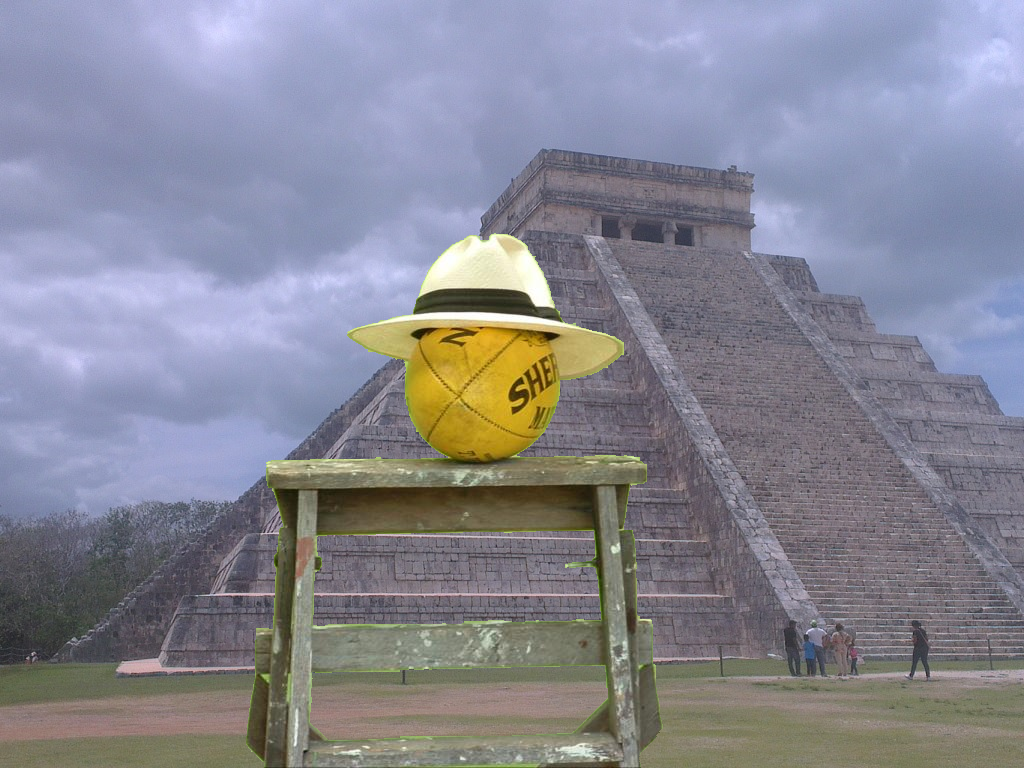
\includegraphics[scale = 0.4]{../images/alpha_matting.png}
		\end{center}
	\end{figure}

	\newpage

	\subsection*{Ejercicio 1}

	\subsubsection*{Descripción}

	Detección de bordes en la imagen.

	\subsubsection*{Solución}

	Primero se cáculo las matrices de derivadas $D_x,D_y$ de cada pixel como se describio en la tarea, usando la convolución de la aproximación de las derivadas con las matrices $k_1,k_2$, cuyo código es:

	\begin{minted}[bgcolor=gray!10!,breaklines]{cpp}
	const int k[2][3][3] = {
		{
			{-1, 0, 1},
			{-2, 0, 2},
			{-1, 0, 1}
		},
		{
			{-1, -2, -1},
			{0, 0, 0},
			{1, 2, 1}
		}
	};
	void Derivates(uchar* image, int* Dx, int* Dy, int imageW, int imageH, int N)
	{
		int index, index1;
		for (int idx = 1; idx < imageW - 1; idx++)
		{
			for (int idy = 1; idy < imageH - 1; idy++)
			{
				index = (idy)*imageW + (idx);
				Dx[index] = 0;
				Dy[index] = 0;
				for (int k_i = -1; k_i < 2; k_i++)
				{
					for (int k_j = -1; k_j < 2; k_j++)
					{
						index1 = (idy + k_i) * imageW + (idx + k_j);
						Dx[index] += image[index1] * k[0][k_i + 1][k_j + 1];
						Dy[index] += image[index1] * k[1][k_i + 1][k_j + 1];
					}
				}
			}
		}
	}
	\end{minted}

	Y después se caculo la ``norma'' de las matrices $D_x, D_y$ para cada pixel para obtener la matriz $MG$ (hay que tener cuidado porque puede ser que este número sea mayor a $255$ por lo que se debe topar) y se usa un umbral de $255/2$ en esta para obtener la matriz $MGT$, con el código:
	
	\begin{minted}[bgcolor=gray!10!,breaklines]{cpp}
	void BordersinImage(int* Dx, int* Dy, uchar* MG, uchar* MGT, int imageW, int imageH, int N)
	{
		int index;
		for (int idx = 0; idx < imageW; idx++)
		{
			for (int idy = 0; idy < imageH; idy++)
			{
				index = (idy)*imageW + (idx);
				if (0 < idx && idx < imageW - 1 && 0 < idy && idy < imageH - 1)
					MG[index] = min(sqrt(Dx[index] * Dx[index] + Dy[index] * Dy[index]), 255.0);
				else
					MG[index] = 0;
				MGT[index] = (MG[index] > 255 / 2 ? 255 : 0);
			}
		}
	}
	\end{minted}

	\newpage

	\subsubsection*{Paralelización}

	\begin{enumerate}
		\item CPU:

		Para la paralelización primero se uso $omp\ parallel\ for\ collapse(2)$, con las directivas $private(index, index1)$ porque cada iteración tiene su propio indice y $default(shared)$ ya que las variables de iteración fueron declaradas localmente y todas puedan accerder a las matrices por multiplicar y al resultado, así los primeros dos for anidados se paralelizaran.

		\begin{minted}[bgcolor=gray!10!,breaklines]{cpp}
	void Derivates(uchar* image, int* Dx, int* Dy, int imageW, int imageH, int N)
	{
		int index, index1;
		#pragma omp parallel for collapse(2) default(shared) private(index, index1)
		for (int idx = 1; idx < imageW - 1; idx++)
		//...
	}
		\end{minted}

		Después se uso $omp\ parallel\ for\ collapse(2)$, con las directivas $private(index)$ porque cada iteración tiene su propio indice y $default(shared)$ ya que las variables de iteración fueron declaradas localmente y todas puedan accerder a las matrices por multiplicar y al resultado, así los primeros dos for anidados se paralelizaran.

		\begin{minted}[bgcolor=gray!10!,breaklines]{cpp}
	void BordersinImage(int* Dx, int* Dy, uchar* MG, uchar* MGT, int imageW, int imageH, int N)
	{
		int index;
		#pragma omp parallel for collapse(2) default(shared) private(index)
		for (int idx = 0; idx < imageW; idx++)
		//...
	}
		\end{minted}

		\item GPU:
		
		Para ello se hizo la alocación y copias de memoria para la imagen fuente, las derivadas de la imagen, y las imágenes MG y MGT:

		\begin{minted}[bgcolor=gray!10!,breaklines]{cpp}
	cudaMalloc((void**)&image, N * sizeof(uchar));
	cudaMalloc((void**)&Dx, N * sizeof(int));
	cudaMalloc((void**)&Dy, N * sizeof(int));
	cudaMalloc((void**)&MG, N * sizeof(uchar));
	cudaMalloc((void**)&MGT, N * sizeof(uchar));
	cudaMemcpy(image, frame.data, N * sizeof(uchar), cudaMemcpyHostToDevice);
		\end{minted}

		Después se uso dos función kernel para calcular las derivadas y las imagenes finales, de tipo $\_\_global\_\_$, con número de bloques y tamaño de malla

		\begin{minted}[bgcolor=gray!10!,breaklines]{cpp}
		dim3 threads(16, 16, 1), grid(divUp(imageW, 16), divUp(imageH, 16), 1);
		\end{minted}
		
		la cuales son

		\begin{minted}[bgcolor=gray!10!,breaklines]{cpp}
	__global__ void Derivates(uchar* image, int* Dx, int* Dy, int imageW, int imageH, int N) 
	{
		int idx = blockIdx.x * blockDim.x + threadIdx.x;
		int idy = blockIdx.y * blockDim.y + threadIdx.y;
		int index, index1;

		if (0 < idx && idx < imageW - 1 && 0 < idy && idy < imageH - 1)
		{
			index = (idy) * imageW + (idx);
			Dx[index] = 0;
			Dy[index] = 0;
			for (int k_i = -1; k_i < 2; k_i++)
			{
				for (int k_j = -1; k_j < 2; k_j++)
				{
					index1 = (idy + k_i) * imageW + (idx + k_j);
					Dx[index] += image[index1] * k[0][k_i + 1][k_j + 1];
					Dy[index] += image[index1] * k[1][k_i + 1][k_j + 1];
				}
			}
		}
	}

	__global__ void BordersinImage(int* Dx, int* Dy, uchar* MG, uchar* MGT, int imageW, int imageH, int N)
	{
		int idx = blockIdx.x * blockDim.x + threadIdx.x;
		int idy = blockIdx.y * blockDim.y + threadIdx.y;
		int index = (idy)*imageW + (idx);

		if (0 < idx && idx < imageW - 1 && 0 < idy < imageH - 1)
			MG[index] = fminf(sqrtf(Dx[index] * Dx[index] + Dy[index] * Dy[index]), 255);
		else if (0 <= idx && idx < imageW && 0 <= idy && idy < imageH)
			MG[index] = 0;
		MGT[index] = (MG[index] > 255 / 2 ? 255 : 0);
	}
		\end{minted}
	\end{enumerate}

	\subsubsection*{Resultados}

	La imagenes resultados son:

	\begin{multicols}{2}
		\begin{figure}[H]
			\caption{MG}
			\begin{center}
				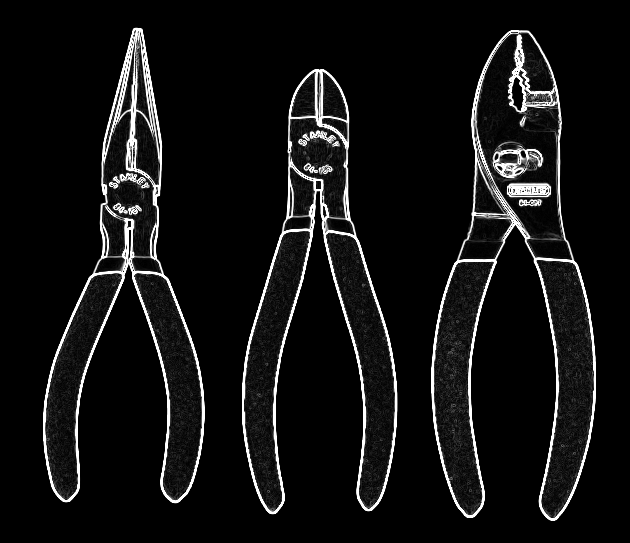
\includegraphics[scale = 0.3]{../images/MG.png}
			\end{center}
		\end{figure}
		\begin{figure}[H]
			\caption{MGT}
			\begin{center}
				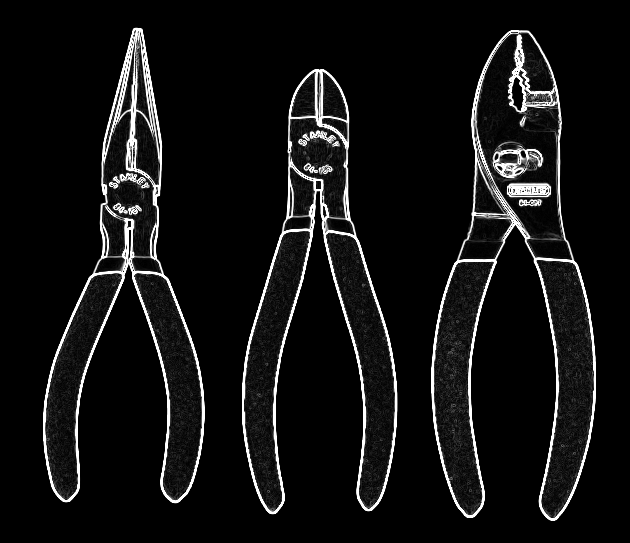
\includegraphics[scale = 0.3]{../images/MG.png}
			\end{center}
		\end{figure}
	\end{multicols}

\end{document}

